\documentclass[a4paper,12pt]{article}

\usepackage[utf8]{inputenc}
\usepackage{color}
\usepackage{epsfig}
\usepackage{float}
\usepackage{graphicx}
\usepackage{hyperref}
\usepackage{ifpdf}
\usepackage{listings}
\usepackage{multirow}
\usepackage{paralist}
\usepackage{subfigure}
\usepackage{times}
\usepackage{url}
\usepackage{xspace}
\usepackage{booktabs}
\usepackage{listings}
\usepackage{srcltx}


\newcommand{\specrule}{\specialrule{1pt}{0.5em}{0.5em}}


\setlength\topmargin{0in}
\setlength\headheight{0in}
\setlength\headsep{0in}
\setlength\textheight{9.5in}
\setlength\textwidth{6.5in}
\setlength\oddsidemargin{0in}
\setlength\evensidemargin{0in}
\setlength\parindent{0.1in}
\setlength\parskip{0.25em}

\ifpdf
 \DeclareGraphicsExtensions{.pdf, .jpg}
\else
 \DeclareGraphicsExtensions{.eps, .ps}
\fi


\newif\ifdraft
\drafttrue

\ifdraft
 \newcommand{\todo}[1]{     {\textcolor{red}  { ***TODO      #1 }}}
 \newcommand{\amnote}[1]{   {\textcolor{blue} { ***Andre:    #1 }}}
 \newcommand{\jhanote}[1]{  {\textcolor{red}  { ***Shantenu: #1 }}}
 \newcommand{\onote}[1]{    {\textcolor{green}{ ***Ole:      #1 }}}
 \newcommand{\fixme}[1]{    {\textcolor{red}  { ***FIXME:    #1 }}}
 \newcommand{\note}[1]{     {\textcolor{red}  { ***NOTE:     #1 }}}
\else
 \newcommand{\todo}[1]{}
 \newcommand{\amnote}[1]{}
 \newcommand{\jhanote}[1]{}
 \newcommand{\onote}[1]{}
 \newcommand{\fixme}[1]{}
 \newcommand{\note}[1]{}
\fi

\newcommand{\lf}{Look-\&-Feel}

\newcommand{\I}[1]{\textit{#1}}
\newcommand{\B}[1]{\textbf{#1}}
\newcommand{\T}[1]{\texttt{#1}}
\newcommand{\BI}[1]{\B{\I{#1}}}

\newcommand{\up}{\vspace*{-1.0em}}
\newcommand{\upp}{\vspace*{-0.5em}}
\newcommand{\dn}{\vspace*{+1.0em}}
\newcommand{\dnn}{\vspace*{+0.5em}}

\newcommand{\OPS}[5]{

  \vspace*{1em}
  \fbox{\begin{minipage}{13cm}
  \begin{tabular}{@{}p{1.80cm} p{1.20cm} p{9.00cm}@{}}
  \B{Objective} & \B{\T{O.#1#2} :} & #3 \\
  \B{Principle} & \B{\T{P.#1#2} :} & #4 \\
  \B{Solution } & \B{\T{S.#1#2} :} & #5 \\
  \end{tabular}
  \end{minipage}}

}

\begin{document}

\title{ \large \vspace{-3.5em} SAGA: An Access Layer to Distributed CI
  and Providing Abstractions for Distributed Applications}


\author{\normalsize Shantenu Jha$^{1}$, Andre Merzky$^{2}$, Ole
  Weidner$^{2}$, \\ \small{\emph{$^{1}$Rutgers University, NJ, 08804,
      USA}}\\ \small{\emph{$^{2}$Center for Computation \& Technology,
      Louisiana State University, USA}}\\ } \date{}
 \maketitle

\ifdraft
 \tableofcontents
\fi

\abstract{The show must go on. Or maybe not in this case..}
 
%%%%%%%%%%%%%%%%%%%%%%%%%%%%%%%%%%%%%%%%%%%%%%%%%%%%%%%%%%%%%%%%%%%%%%
% 
\section{Introduction}
 \label{intro}

% \begin{verbatim}
%    - Grand intellectual challenges of designing DCIs
%      - how to design infrastructures to bridge gap
%      - what is role of abstractions/interfaces in general, and for
%        SAGA
%        - interface necessary, but sufficient?
%        - should be sufficient, if fully functional (contract)
%        - but what are the challenges of providing a functional interface?
%        - at the end deep integration!
%        - from there follows design, limitations
%          (possibly goes partially into conclusions)

%     - roles for SAGA: 
%       - shield from environment
%       - need to be able to reason about distribution without
%       considering those env details

%     - Limitations of SAGA:
%      -- APIs are never enough! The challenge of implementing them. 

% \end{verbatim}

DCI such as TeraGrid (and now XSEDE) have tremendous potential for
science and engineering, and impressive advances notwithstanding,
there have only been a limited number of applications that have been
successful in exploiting the collective capacity of DCI.  Innovative
and novel usage of DCI has generally not kept pace with other
technical advances of DCI; an analysis of the usage modes of
applications using the TeraGrid (in its final year of operation before
it transitioned to XSEDE) substantiates this
observation~\cite{katz-usagemode}. There are several underlying
reasons that explain the status of affairs: developing large-scale
distributed applications is fundamentally a difficult
process~\cite{dpagrid2009, dpa-surveypaper}, made more difficult due
to the scarcity of high-level abstractions (system and
application-level) and interfaces that bridge the divide between the
needs of applications and the functionalities offered by middleware
and system-level capabilities~\cite{saga_data_intensive_abstractions}.
Deployment and execution concerns are often disjoint from the
development process~\cite{dpagrid2009}, in that functionally
incomplete solutions and not end-to-end solutions are provided to the
scientist.

% Admittedly, many are non-technical, such as policy,
% allocation, etc., however, a fundamental technical challenge is the
% need to support a broad range of application use-cases and usage
% modalities on a range of platforms with varying performance
% constraints. 

Against this backdrop, the distributed infrastructures available to
scientists continue to evolve in scale, technology, as well as
capability.  Investments in legacy applications need to be preserved,
while at the same time, development of functionally novel and
architecturally different applications for new and evolving
environments needs to be facilitated.  This fundamental mismatch
between requirement of DA and capabilities of DCI is one of the
intellectual problems that this paper will address.



% Developing versus Deployment versus Using

Improvements in algorithms, numerical methods and Moore's Law have
enabled computing to contribute to major advances in Science \&
Engineering (S\&E). In spite of impressive growths from each of these
factors however, in order to effectively solve the next-generation of
S\&E challenges, more computational capacity will be required than is
typically available locally, whilst concomitantly being able to
utilize the increasing computational capacity in novel and interesting
ways. This suggest the need for a advanced, balanced and comprehensive
cyberinfrastructure (CI) --- comprised of software layers (the
application capabilities, tools and services) and physical layers
(grids, clouds, special purpose architecture and ``vanilla''
high-performance machines/clusters), along with scalable approaches to
utilize the CI.

One way to provide the CI that can support novel usage modes and
scaling --- scaling-out (the number of tasks) as well as scaling the
number of resources, is to federate computing resources.  Federation
here refers not just to machines, but also services and tools.  The
federation of previously independent and individual resources, results
in extensible and scalable capabilities that are more powerful than
the simple sum of its parts.  The set of techniques and technologies
used to federate resources is collectively called Grid Computing.

Although federating resources is a great way to scale the number of
resources usable, all too often the resources being federated are
owned, operated and designed for different applications and usage
modes, and thus inherently different. Federation therefore introduces
the challenge of interoperability, arising from heterogeneity and
complexity in software stacks, policies and resource performance, all
of which result in barriers to interoperation at both the system and
application levels.

In addition to enabling federation --- and thereby scalability and
extensibility, additional design objectives that are fundamental to
distributed applications and capabilities are portability and
interoperability.  One approach to addressing these persistent and
fundamental challenges of enabling applications and capabilties to
interoperate across federated heterogenous DCI has been to design and
develop a simplified interface to DCI which serves as an access layer
to DCI as well as providing the base abstractions upon higher level
capabilities can be built. A specific instance of such an
interfrace--- known as SAGA --- the Simple API for Grid Applications,
provides frequently required and used functionality, such as remote
job-submission, remote file/data transfer, remote coordination, etc.,
to construct applications capable of utilizing distributed federated
CI.

Given the landscape of DCI, the design objectives of distributed
applications and capabailities, a fundamental and challenging research
agenda emerges: how can distributed applications and capabilities
(tools, frameworks etc) be designed and developed so as to adhere to
the set of design objectives.  This is the intellectual problem that
lies at the heart of this paper as well as the research agenda
manifested by the SAGA project.


% The process of designing and deploying large-scale DCI such as XSEDE
% and OSG, presents a critical and challenging research agenda for CI
% developers.


% Distributed applications utilize multiple resources, or are capable of
% utilizing them. One could argue that any application that would
% benefit from increased peak performance, throughput, or reduced time
% to solution, by using multiple compute and distributed data resources,
% can be classified as a distributed application, or a candidate to be
% formulated as such.
 
% For context: it is still very difficult to develop a distributed
% application that can use O(1000) processors, transfer/handle O(100) GB
% data and use O(10) arbitrarily chosen sites, repeated over 10
% arbitrary chosen days. The only science projects that can do so
% currently are Big Science projects, with very large teams and levels
% of effort.  Individual PIs/scientists are unable to do so, but there
% are many who clamor and need to be able to do so.


%%%%%%%%%%%%%%%%%%%%%%%%%%%%%%%%%%%%%%%%%%%%%%%%%%%%%%%%%%%%%%%%%%%%%%
% 

\section{Background and Motivation}

\subsection{Landscape of DCI}
\label{ssec.dci.landscape}

\subsubsection{The complexity of DCI}
\label{ssec.dci.complex}

\subsubsection{DCI Challenges: Infrastructure Perspective}

  It is well known engineering practice to keep systems as modular and
  simple as possible, as those attributes are major indicators for
  maintainability and stability.  Simplicity is also a significant
  contributor to ease-of-use.  DCIs are, of course, designed with
  those objectives in mind -- so, why do they appear to be inherently
  complex, fragile, and difficult to use?

  The reasons are manifold, and not always obvious.  First, unlike
  many commercial IT infrastructures, academic DCIs tend to serve a
  considerably large, and importantly \I{diverse}, set of user
  communities.  In particular, this diversity of users and use cases
  imposes a large number of functionality requirements on the DCI --
  and those requirements are often not well specified, or are expected
  to evolve over the lifetime of the DCI.  Those requirements in turn
  imply a large number of design constraints, which are sometimes even
  contradictory.  That makes it basically impossible to come up with
  \I{simple} DCI software stacks.  Along the same lines, the
  heterogeneity, which is inherent to DCIs on many layers, including
  the hardware resource layer, is also a reflection of the large and
  diverse set of use cases and user communities.

  The modularity of the stacks should actually be encouraged by the
  large set of functionality requirements -- on the first glance, that
  seems to be the only viable option to manage those requirements in a
  scalable and evolvable way.  But there are several boundary
  conditions which act diametrical to the modularity principle.

  First, academic software is rarely designed from scratch, but rather
  grown.  That may not hold true for individual elements of the stack
  (although it often does), but it certainly holds true for the DCI
  stack as a whole.

  Secondly, very few software components are backed by a sustained
  software support and maintenance model -- instead, the usual
  approach of funding software in small, very finite chunks (called
  projects), results in software that is, once the project concludes,
  in limbo.  The notion of follow-up and integration projects exists,
  of course, which try to address exactly that problem, but those
  projects are rare, and also finite and short.  In general, the
  current scheme of software funding favors research level software
  over production level software -- maintenance and sustainability are
  often an appendix in project proposals, and not the core.  Funding
  agencies have begun to realize the problems with that approach --
  but it will need significant time and culture change to address it.

  Thirdly, academic DCIs are very often not centrally controlled.
  Instead, they frequently represent a federation of relatively
  independent resource providers, which work together toward a common
  (set of) goal(s).  That is in sharp contrast to commercial IT
  infrastructures, where heterogeneity and autonomy can, at least
  in principle, be controlled at any level.

  % Finally, there is ego.  Well, plural, there are egos, which is
  % exactly the problem.

\begin{verbatim}

Why are DCIs complex in the first
place?  Many requirements, many different usage modes, no simple
straight-forward solution (i.e. engineering approach) possible.
Plethora of point-wise solutions vs. end-to-end solutions
 

DCI is not just scaling up a single computing resource. DCI is
complex: heterogeneous software, access-layers, policy.. 
An engineering challenges. 
Difficult to integrate services \& software (Service-level Interop)
Middleware: Heterogeneity and semantic incompatibility

This is not Google where a top-down solution, as much of a sociocultural
challenge as a technical one. Slow/lack of agreement towards
a standards-based software
 
Fundamental: How to design and implement DCI such that the
whole is greater than the sum of the parts? (where each of the parts
is complex heterogeneous systems!!)
 
DCI: Difficult to use for (domain) scientists, Complexity O(N), likely worse

Narrow grids vs. broad grids: narrow grids provide a more limited set
of solutions (cater to more limited set of requirements), and can thus
potentially be implemented on a lower complexity level.

\end{verbatim}


\subsubsection{DCI Challenges: Application Perspective}

\begin{verbatim}

End-to-end application support missing

Many moving and changing parts insufficient / partial coverage

Complex coordination requirements; How to manage coordination?

Well defined interfaces; Standard-layers handle hard parts, 
allowing innovation elsewhere

Abstractions Support: Where, when, how to distribute? 

Both Development and System/Infrastructure level abstractions

Effective Dynamic resource utilization and execution models
Beyond simple static single batch-mode

\end{verbatim}

 A distributed application has some unique challenges: a distributed
 application/developer has to reason about the environment that the
 application will execute in, has to make assumptions about the
 runtime availability, and has to assume a failure model that
 transcends complete knowledge of the application or even predicates
 it upon knowledge of a system/resource.  Whereas the choice of tools
 will always be influenced by soft factors, the challenge for us is to
 think of abstractions that enable the developer to reason about the
 above hard factors, and not just the tools, services and
 capabilities.

 The process of developing and deploying large-scale distributed
 applications presents a critical and challenging agenda for
 researchers and CI developers.  In spite of the tremendous potential
 of distributed systems, there have only been a limited number of
 successful distributed applications; in the case of the TG, where
 there has been success, the effort required has been {\it heroic} but
 unsustainable and thus not surprisingly heavily biased towards big
 showcase projects. It is difficult to examine under the covers of
 these prestige projects, but there has not been a trickle down
 advantage to communities of smaller users, who cannot sustain heroic
 efforts in order to accomplish their science.


 \jhanote{Some text about the mismatch between DCA requirements and
 DCI capabilities}



%%%%%%%%%%%%%%%%%%%%%%%%%%%%%%%%%%%%%%%%%%%%%%%%%%%%%%%%%%%%%%%%%%%%%%
% 
\subsection{Access Layers to DCI and Abstractions for DA}\todo{AM, SJ}
\label{ssec.dci.access}

Revisiting the reasons why production DCI have not been used in more
innovative ways, reveals that there are currently gaps at several
levels: application development and runtime capabilities, as well as
system software and deployment support~\cite{dpagrid2009}.  No single
solution can address gaps at all levels, or for the entire spectrum of
applications.  

We posit, however, that a well-defined, stable general purpose API is
one critical element of the solution, as that exposes the basic
distributed capabilities to serve as an uniform access layer to the
infrastructure layer as well as a building blocks for higher-level
applications, capabilities and tools.

We will substantiate this claim from two different
viewpoints/directions: in the first, we will examine the role of an
API that acts as an Access Layer to the levels/layers of
infrastructure beneath. The second viewpoint will examine how we can
build tools \& services using such an API...

The vertical axis can be thought of as a non-continuous ordering, with
the bottom level being closer to the hardware and the upper levels
being closer to the application.

It is important to note that every API can be considered as an
abstraction to underlying layers: the first challenge when designing
an API the challenge is to define the level for such an abstraction
layer.  

It is often misunderstood that placing an abstraction level at a given
level, implies that all capabilities below that level should be
supported. However this is not the case, and a second challenge is to
define the scope, viz., which features and capabilities should the API
provide an abstraction too.

\jhanote{This section should result in the motivation of the API:
  level and scope}

%\jhanote{Q: Determine whether HG metaphor is 2 dimensional or 3?}

\begin{verbatim}
   - Role of an Access Layer as defined:
      - provide abstractions to set-of/selected levels/capabilities below
      - support heterogeneity, environment (elaborate on environment..), 
      - provide uniformity

    - Role for the abstraction to DA 
      - need to be able to reason about applications without 
        considering those environment details

   - Placement of the neck, and width/scope of the HG.
     Placing the access layer/level-of-abstraction/where is the neck
     of our hour glass?

   - Define where it is placed. THAT IS SAGA...
\end{verbatim}

\subsection{Related and Prior Work}
%%%%%%%%%%%%%%%%%%%%%%%%%%%%%%%%%%%%%%%%%%%%%%%%%%%%%%%%%%%%%%%%%%%%%%
% 
\section{Design Objectives and Principles for SAGA as an DCI Access layer}
\label{sec.obj}

 \amnote{needs introduction, purpose} \amnote{SAGA API specification
 vs. SAGA implementation vs. SAGA project etc. -- need to be defined
 /  separated here or before}

 Objectives for SAGA are drawn from both its role of access layer, and
 its role as an abstraction and building-block for Distributed
 Applications, i.e. as a component of the DCI software stack -- thus
 there are such objectives which apply to the API scoping and
 specification, and such that apply to its implementation aspects.

 The SAGA API specification process and the SAGA API implementation
 efforts have been relatively synchronous, but do in fact follow
 a quite different and sometimes contradictory set of objectives.  The
 following subsection will first discuss objectives relevant to the
 specification, and later those relevant to the implementation of the
 SAGA API.
 
 \fixme{above is incomplete and repetitive}



 \subsection{Design Objectives}

  % should fall out from section 2!

  SAGA (the API, including its extensions, language bindings and
  implementations) is ultimately designed to address some of the DCI
  challenges discussed above, and in particular those which are faced
  by users and developers of distributed applications for those DCIs.
  Starting from that premise, the design of SAGA follows from a number
  of related constraints and design objectives.


  \subsubsection{Objectives for the SAGA Specification Design}
  \label{sec.obj.spec}

   \amnote{we do not derive standardization as an objective :-P}
   \amnote{intro, source and purpose of these objectives}

   \subsubsection*{Managing System Heterogeneity}
   \label{ssec.obj.heter}

    % O: manage system / middleware heterogeneity
    % P: abstraction(?) of heterogeneity
    % S: abstract API, adaptors to implement abstractions
    %    (worked out in principle, devil is in details, compliance tests
    %     missing on adaptor level)

    The overarching motivation to attempt a project like SAGA in the
    first place is to make DCI system heterogeneity manageable,
    specifically for the programmer of distributed applications.
    There are different ways to achieve that -- but a very common
    principle is 'Abstraction': the heterogeneous components are
    exposed via an abstract (and apparently homogeneous) interface
    layer, which exposes the underlying system diversity in a uniform
    way.

    In general, it is \B{much} simpler to provide syntactic
    abstractions than semantic ones.  Syntactic abstractions, which
    map specific syntactic constructs onto others, while completely
    maintaining the semantic properties, in most cases boils down to
    an engineering exercise.  For example, an programmatic API can
    with relative ease be exposed as a command line interface, and
    vice versa.

    Semantic abstraction usually is, however, more complex: any
    semantic differences between two heterogeneous components must be
    handled, and either (i) must be equipped with mechanism to achieve
    semantic compatibility, or (ii) must be removed from abstract
    interface, or must (iii) be documented as being backend specific.

    Approach (i) can be extremely difficult -- it requires the
    abstraction layer to implement parts of the lower level system's
    semantic as needed -- but those lower levels are complex, as 
    discussed earlier, so that is a very difficult task, which is hard
    to scope.  Removing the capability from the abstraction (ii) is a
    relatively simple way, and works well for capabilities which are
    rarely needed -- but defining what parts are \I{really} needed and
    what parts are not is extremely difficult, and can in fact change
    over time.  Also, leaving too many small pieces off diminishes the
    usability of the overall abstraction.  And (iii), allowing backend
    level semantics to leak through the abstraction layer, is
    obviously a last resort, as it defeats the very purpose of the
    abstraction.

    The approach of the SAGA specification is to (a) base the API on a
    set of explicit use cases, best practices and existing standards
    to define the semantic target scope as tightly as possible and in
    an extensible manner (relates to (ii) from above), and (b) require
    the API implementation to use any required mechanisms to provide
    semantic compatibility with the API specification (relates to (i)
    from above).  Implementations are only allowed to break semantic
    compatibility in exceptional cases, and must document those
    exceptions.


    \OPS{S}{1}
    {manage system heterogeneity}
    {abstractions}
    {abstract API, tight semantic API scope, mandatory API semantics}

    \onote{the term 'abstract API' is somewhat overloaded and should be avoided.}

   \subsubsection*{Ease of Use}

    % O: ease of use
    % P: top-down
    % S: use cases, extensible API, 80:20
    %    (worked out in principle, moving targets, ease of use is more
    %     than simple API (ease of implementation is orthogonal, but
    %     related)

    Another very obvious objective of the \B{S}AGA specification is to
    define an API which is simple and intuitive to use (while not
    being semantically trivial).  In that respect, the design
    basically follows the mantra of Larry Wall \I{"make easy things
    easy, and hard things possible"}: the scope definition discussed
    above (a) was used to focus the design on the mostly used elements
    which are semantically the least ambiguous between different
    backends.  Interestingly, that very often turned out to be
    elements which to not have a clear functional representation on
    the systems in question, but instead are orthogonal issues, such
    as asynchronous operations, and security management related issues
    (see also subsection~\ref{ssec.bestpractices}).  It is thus not
    surprising that the so-called non-functional part of the SAGA-API
    (also called the SAGA \I{Look-\&-Feel}) occupies a relatively
    large part of the overall SAGA API specification.

    Another principle used in order to fulfil that objective is to
    heavily lean on existing standards and best practices, and to
    reference or use them where possible.  Examples for this are:
    futures for asynchronous operations, JSDL and DRMAA for job
    descriptions, POSIX for file system (and similar) operations, BES
    for job state management, etc.  That approached served in fact two
    purposes: it made semantic matching to the system level easier and
    more consistent, as it was likely that those systems followed the
    same standards and best practices, and also made the API simpler
    to use, as users met well known and accepted paradigms they new
    how to handle.

    \OPS{S}{2}
    {ease of use}
    {"make easy things easy, and hard things possible", 
     reuse of standards and best practices}
    {separate 'orthogonal' API elements, reuse existing standards,
    built upon previous work}

   \subsubsection*{Manage Complexities}
   \label{ssec.obj.compl}

    % O: manage complexities (needs good scoping, sect. 2)
    % P: compartmentalization, abstraction(?)
    % S: loose coupling                (only partially sucessfull)
    %    avoid leakage of abstractions (only partially sucessfull)
    
    % --> define heterogeneity and complexity in sec. 2
    % --> also discuss what abstraction means in sec. 2

    Ultimately, most of the engineering challenges in distributed
    systems (and often also in non-distributed systems) is to manage
    complexities.  This section specifically targets the application
    level efforts to handle system level complexities.

    Historically, distributed systems have often be considered as
    federations of relatively independent resources, connected via
    mutually agreed interfaces.  That leads to very heterogeneous, but
    also very flexible infrastructures.  But also, that approach
    leaves it mostly to the upper layers (middleware services, tools
    and applications) to handle the resulting mess, aeh, system
    complexity.  The middleware layer in turn is in many cases, at
    least for academic DCIs, also a federated mix of different
    services, policies and capabilities -- which in turn leaves it to
    the tooling and application layer to catch much of the system
    complexity.  This is often not reasonable possible for academic
    software projects, at least not in a portable and sustainable
    fashion.  As a result, many excellent developments have been
    constrained to a small subset of DCI resources, or use complex,
    volatile ad-hoc solutions.  Only comparatively large research
    projects, such as iRODS, or large international collaborations,
    such as CERN, managed to compartmentalize specific pain-points,
    and to provide at least point-wise solutions.

    \amnote{we do not define what the system complexity really is.}

    There are well established software engineering principles which
    would allow to address the system complexity problems, such as
    component based software development, well defined
    abstractions\footnote{As always with abstracting layers, it is a
    challenge to avoid the leaking abstractions.}, standardized
    interfaces and protocols.  Many of those principles should be (and
    are) applied on the middleware layer -- but some also apply to the
    application and tooling layers.  

    With that background, the SAGA API strives to define semantically
    \B{rigid} abstract constructs, which shields higher (than SAGA)
    layers from much of the syntactic and semantic complexity.  Also,
    the SAGA API is designed to encourage implementations which base
    on loose coupling of components, and which can compartmentalize
    the interactions with the lower level environments.

    \OPS{S}{3}
    {manage complexities}
    {software engineering principles, standardization, abstractions}
    {rigidly define API constructs, in both syntax and semantics,
    modular API design, encourage loose coupling implementations}


   \subsubsection*{Cover Common Usage Patterns}

    % O: cover commonality on application levels (pattern? frameworks?
    %    What is the application?  Semantic coverage...)
    % P: abstraction, pattern
    % S: high level API, use case driven, known models etc.

    A repeatedly listed requirement to SAGA was to \I{"make commonly
    used functionality simple"}.  While the SAGA use cases listed
    a number of those commonly used functionality, it remains
    a challenge to identify suitably general higher level
    abstractions.  One has to keep in mind that the higher the
    abstraction level, the smaller is the semantic scope of that
    abstraction.  Thus, the higher the abstractions provided, the
    lower the flexibility and generality of an API.

    Instead of placing the SAGA API on the level of high level
    programming pattern or frameworks, it seemed advisable to instead
    place it on a relatively low abstraction level, while making it
    easy to build such more abstract patterns and frameworks on top of
    SAGA.  For example, SAGA provides mechanisms to run and track
    individual job instances, mechanism to store application state,
    and mechanisms to coordinate application components.  Those
    functionalities make it relatively simple to implement, say,
    a stateful master-worker framework, which is one of the more
    commonly used programming patterns for distributed applications.

    At the same time, SAGA is generally placed on a higher abstraction
    level than the underlying native middleware interfaces --
    semantics which is internal or specific to individual middleware
    types or instances are generally not exposed via SAGA.  That
    avoids the leakage of non-portable middleware abstractions to the
    application layer (see also~\ref{ssec.obj.heter}
    and~\ref{ssec.obj.compl}).

    \OPS{S}{4}
    {cover common usage patterns}
    {"make commonly used functionality simple"}
    {use case driven design, balance of higher level abstractions
     versus semantic expressiveness, recognisable and intuitive
     abstractions and patterns}


  \subsubsection{Objectives for the SAGA Implementation Design}
  \label{sec.obj.impl}

   The previous set of objectives were identified even before the
   scoping and definition of the SAGA API specification started -- as
   such, they are mostly focused on the idealistic notion of an access
   layer API.  When dealing with SAGA as a code base, a community
   project, a software deliverable, and as a component of some DCI,
   a complementary set of design objectives arises -- which lead to
   stringent constraints on the SAGA architecture and software
   development cycle.


   \subsubsection*{Implementation Sustainability}
   \label{ssec.obj.sustain}

    % O: implementation sustainability
    % P: simple implementation, community effort
    % S: modular implementation with good tooling support,
    %    open source, community support, project identity

    % O: stability (code, usage)
    % P: software engineering...
    % S: standardization, modularization, release cycles, ticket 
    %    responses, certification, pre-deployment
    
    Academic software projects are usually planned out for the
    duration of a project funding period.  In some cases, long term
    commitments of funding agencies and/or commitment of project
    independent institutional funds allow a more long term planning --
    but that is a relatively rare exception.

    Further, academic software development is often considered to be
    a secondary to the academic research a project targets -- again,
    relatively rare exceptions exist where software development itself
    forms the explicit target of a funded project.

    Finally, discontinuity of staffing in academic environments
    (Students graduate and leave, PhD get completed and people move
     on, etc), lead to discontinuities in code ownership, a situation
    which is aggravated by the frequent lack of a coordinated and
    scalable approach to software documentation, packaging and
    deployment.

    These (and other) circumstances make software sustainability
    a challenge in academic environments (and arguably in others,
    too).  Nevertheless, for a relatively generic, infrastructure
    independent DCI access layer, software sustainability is crucial.  

    A number of approaches and best practices  exist to support
    software sustainability in academic environments, to some extent.
    Foremost of all, the chances of survival for a given software
    product increases dramatically with the rate of its uptake, and
    the number of code contributing parties (Open Source is a widely
    accepted development model in academia).  Code simplicity,
    modularity, portability and tooling support are properties which
    support project-external contributors and users.  Also,
    early adoption and increasing uptake (by users and other projects)
    increases the chances for continued funding.

    Last, but not least, an open development process and the
    integration of that development process in the open source
    ecosystem are considered vital for the sustainability of the SAGA
    code base.

    \OPS{I}{1}
    {implementation sustainability}
    {implementation simplicity, community effort}
    {code simplicity, modularity, ease of contribution, tooling
    support, early adoption, open process}



   \subsubsection*{Manage System Heterogeneity}
   \label{ssec.obj.system}
    
%     complex deployment and runtime environment
%     O: manage system heterogeneity (on SAGA / impl level)
%     P: loose coupling (software engineering), integration!
%     S: lightweight deployment, low dependencies, 
%        pre-packaging + certification
%        (software vs. system heterogeneity)

    As discussed in subsection~\ref{ssec.dci.complex}, the wide range
    of target usage modes for academic DCIs leads to a proliferation
    of software stacks and software configurations and combinations,
    and thus to a significant system heterogeneity.  Ensuring
    syntactical and semantical software portability, i.e. to ensure
    that software is usable in different environments and is also
    fully and consistently functional in different DCI contexts, is a
    non-trivial problem.  Again, a number of software engineering
    techniques target that problem space, such as the encouragement
    toward a modular software architecture with loosely coupled
    components; a low degree of internal and external software
    dependencies; portable code base; well defined and automated
    procedures for packaging, testing, deployment and possibly
    certification.

    Note that heterogeneity has also been discussed above, in the
    context of the API specification objectives.

    \OPS{I}{2}
    {manage system heterogeneity}
    {software engineering principles}
    {loosely couples components, low degree of external dependencies, 
    software portability}


   \subsubsection*{Scalability}
   \label{ssec.obj.scalability}

    % Scale-Up:     add resources to a single node / instance
    % Scale-Out:    add nodes / instances to the application
    % Scale-Across: scale out across multiple distinct resources
    %
    % O: scalability (code, usage, performance)
    % P: extensibility, software engineering principles
    % S: modular code base, low overhead, no hard limits,
    %    impl constraints orthogonal to scalability approaches

    \fixme{need to define scale-up, scale-out, scale-across somewhere
    before.}

    \fixme{ref in spec section 4, for non-functional API}

    There are multiple reasons why DCI are amongst the prevalent IT
    infrastructures for scientists (see
    subsection~\ref{ssec.dci.landscape}), but supporting scalability
    is prominent amongst them.  Not only that a single application
    instance can scale-out over the large resources available on DCIs,
    but also that applications and projects can scale across a diverse
    set of resources, and eventually across distinct national and
    international DCIs.  In fact, as different DCIs often feature
    different capabilities (for example, HTC on OSG vs. HPC on XSEDE
    vs. Data centric computing on DataNet), the scale-across is an
    ability required by a few, but important set of applications.
    \fixme{examples, refs}

    In order for SAGA to support application scalability the SAGA
    layer itself must not become a performance or scalability
    bottleneck.  It needs to be designed and implemented such that it
    does (a) not incur any significant additional runtime or memory
    overhead in its own (scale-up), (b) that it supports the addition
    of application threads, processes and components (scale-out), and
    (c) that it supports the concurrent access to different resources
    and DCIs from within a single application instance (scale-across).

    \OPS{I}{3}
    {scalability}
    {orthogonal design}
    {no interference with orthogonal elements which are required for
    different scalability aspects}


   \subsubsection*{Supporting SAGA Usage Modes}
   \label{ssec.obj.usage}
    
    % O: multiple levels of use of SAGA (API coding, tools, higher up)
    % P: packaging, 'extensible' code, 
    % S: integration on different levels (application / tooling level)
    %    -- spectrum of applications is broad...
    
    S\B{A}GA is, by definition, an API.
    Subsection~\ref{ssec.dci.acess} discussed the different options
    for DCI access layers, and motivates an API access layer as the
    most suitable approach.  However, other access layer approaches
    also provide significant benefits for a diverse set of use cases,
    and usage modes.  Not surprisingly though, it is possible to
    construct a variety of access abstractions -- such as command line
    tools, gateways, portals, or hight level frameworks -- on top of
    the SAGA API.  It is a design objective of SAGA as a software
    product to support the creation of such access layers, by
    documentation, tooling, and integration mechanisms.  The
    previously listed extensibility objective (see ???) is also
    relevant for the support of additional usage modes.

    \OPS{I}{4}
    {support different usage modes}
    {multi-level approach}
    {extensible specification and implementation, good tooling
    support, multiple levels of abstractions}


%     - challenge of environment (define env: fragile, lossy, heterog,
%       reliability/failure, complex, dynamic, evolving, ) 
%       - adaptors: approach to heterogeneity (different syntax, different
%         semantics, late binding, heterogeneous in time -> dynamic), also supports 
%         separation of concern
%       - reliability: model exists (define it), but is addressed elsewhere
%       - continuous testing is part of the answer to dynamic env /
%         boundary condition
% 
%     - challenge of diverging and multitude of application
%       requirements?
% 
%      -> be relevant for large user base and longish time scales
%      -> good scoping API, use cases, requests, common practice
%      -> still too large, apps are moving, no 1st principle apps,
%         stability vs. agility, poorly understood use cases, moving targets, 
% 
%     - tight coupling, leaky abstractions
%   
%      -> extensibility
%      -> adaptors, packages, higher level abstraction
%      -> adaptors: hard to enforce semantic coherence
%         packages: ok (mod impl)
%         HLA:      hindered by impl deficiencies
%   


 \dn\hrulefill\\
 \fixme{not sure why the paragraph below is right here - should be
 moved IMHO?}

 {\it The objective of SAGA, the 'Simple API for Grid Applications is
 to provide this missing critical component in the distributed
 cyberinfrastructure ecosystem.}\footnote{While the API's name
 suggests its string ties to Grid based DCIs, it is in fact a general
 purpose API for distributed -- which is historically rooted in the
 Grid community.}  SAGA can provide effective abstractions that can
 hide the environmental complexity, supplement the incompleteness and
 lack-of-extensibility of many tools used whilst promoting
 interoperability as first-class design objective.  On the other hand
 it must provide the building blocks upon which the distributed
 applications, tools and frameworks can be built...

\jhanote{This section should end up motivating the Architecture and
 Implementation}


%%%%%%%%%%%%%%%%%%%%%%%%%%%%%%%%%%%%%%%%%%%%%%%%%%%%%%%%%%%%%%%%%%%%%%
% 
\section{Design and Structure of the SAGA API}
\label{sec.api}

 The SAGA API (as in API specification, not implementation) has been
 designed with the background of objectives described in
 section~\ref{sec.obj.spec}.  This section describes the
 general structure and scope of the API, and demonstrates how that
 scope facilitates the implementation of distributed applications,
 frameworks and tools.

 The SAGA API structure is best understood when discussing it in
 different perspectives: general distributed programming practices,
 and specific distributed operations semantics.

 \subsection{General Distributed Programming Practices}
 \label{ssec.bestpractices}
 
  The prevalence of distributed programming in the fields of
  scientific computing and computational engineering led to a large
  body of collective best practices and successful programming
  techniques.  Obviously, the SAGA API is expected to build upon those
  where possible and sensible, and to nicely interact with those
  orthogonal to the API itself.  Among them are, for example:

  \begin{itemize}

   \item asynchronous operations,
   \item event based programming,
   \item multithreading and concurrent execution, 
   \item caching (or latency hiding in general), 
   \item eventual consistency, and 
   \item separation of syntax and semantics\footnote{For example, most
         distributed communication models separate transport layer and 
         protocol layer.  Another example is the separation of data 
         formats and data models.}.
  \end{itemize}

  In order to separate the API design considerations in respect to
  these best practices from the actual semantic scope of the API, the
  SAGA API specification consists of two parts.  First, there is a so
  called 'functional' part of the SAGA API, which, organized into
  several API packages, spans the semantic scope of the API.
  Secondly, there is a so called 'non-functional' part -- whereas the
  latter name is probably not a fortunate choice, that is the part
  which addresses general distributed programming concerns as
  mentioned above, and is applied across all 'functional' packages.
  That mechanism provides a common look-and-feel to those 'functional'
  packages, which is particularly important as the API allows for API
  extensions in the 'functional' area.

  The 'non-functional' part of the SAGA API describes how SAGA
  operations are rendered for asynchronous executions modes, how
  asynchronous notifications are rendered, how security tokens are
  specified, how error conditions from different backends are
  uniformly managed, how the SAGA API behaves in multi-threaded
  environments, etc.

  As an example, the code (here in C++) in listing.~\ref{code:async}
  shows how an asynchronous file copy operation is rendered in SAGA --
  the very same mechanism (create a stateful task object for that
  operation) is applicable to \I{any} SAGA API operation -- the
  asynchronous part of the SAGA API is \I{orthogonal} to the
  'functional' part of the SAGA API.\\

  \begin{lstlisting}[language=c++,
                     basicstyle=\footnotesize\ttfamily,
                     keywordstyle=,
                     numbers=left,
                     numbersep=1em,
                     showstringspaces=false,
                     frame=single, 
                     label=code:async,
                     caption=SAGA API Code example for asynchronous
                     operations (in C++),
                     captionpos=b]
 saga::filesystem::file f (source_url);
 saga::task t = f.copy <saga::task::Async> (target_url);

 while ( saga::task::Running != t.get_state () )
 {
   // do something useful
 }

 if ( saga::task::Failed != t.get_state () )
 {
   std::cout << "file copy failed: " << t.get_error ();
 } 
 else
 {
   std::cout << "file copy done " << std::endl;
 }
  \end{lstlisting}
\onote{Let's discuss if code blocks really necessary?}

 
 \subsection{Semantic Scope of the 'functional' SAGA API}

  The 'functional' scope of the SAGA API was derived from a set of use
  cases, and thus is defined by the set of semantic operations
  considered essential and beneficial to the programming of typical
  distributed applications.  Additionally, the API layout is oriented
  on other well-known APIs and standards, such as POSIX, Java CoG,
  GAT, GridRPC, DRMAA, JSDL and others.

  The problem with that approach is, (i) that applications outside the
  set of considered use cases may require slightly or significantly
  different functionality, and (ii) that APIs and paradigms on which
  the SAGA specification was based are not widely used anymore, which
  makes that similarity of limited value.

  To address these problems, the API's scope was widened in an attempt
  to cover related or likely functionality.  For example, the use
  cases defined a strict requirement to the API to provide a
  \T{file.get\_size()} method -- the API definition thus attempts to
  provide reasonable support for other POSIX \T{stat()} information
  items.  For most parts, that approach worked reasonably well -- but
  it also led to some pollution of the API with semantics which has so
  far not been used, and/or has been difficult to implement.

  To further accommodate new use cases with significantly different
  semantic requirements on the SAGA API, the API was designed to be
  extensible by new 'functional' packages, while encouraging to define
  those new packages on top of existing packages.

  The approximate functional semantic scope of the API is listed in
  table~\ref{tab:apiscope}.

  \begin{table}[h!]
   \begin{footnotesize}
   \begin{center}
     \begin{tabular}{@{}p{2.80cm} p{3.50cm} p{9.50cm}@{}}
      \toprule
        {\bf Package} & {\bf Related APIs / Standards} & {\bf Scope} \\
        \multicolumn{3}{@{}l}{\B{Saga Core API}}\\
      \specrule
        Jobs         
        & GRAM, BES, DRMAA,\newline GAT, JSDL
        & \T{job description, create, suspend/resume, state, cancel,
        inspection, stage-in/out} 
        \\
      \midrule
        Namespace     
        & POSIX, GridFTP, GAT 
        & \T{open, close, create, copy, move, delete}
        \\
      \midrule
        Files         
        & POSIX, GridFTP, GAT 
        & \T{stat, read, write, seek, scattered I/O, pattern based I/O, extended I/O} 
        \\
      \midrule
        Replicas
        & Globus, SRM, Raptor, GAT
        & \T{list/add/remove/update\_location, replicate, annotate,
          search}
        \\
      \midrule
        Stream
        & POSIX, BSD, XIO, GAT
        & \T{serve, connect, close, read, write, wait}
        \\
      \midrule
        RPC
        & RPC, GridRPC
        & \T{open, call, in/out/inout parameter}
        \\
      \specrule
        \multicolumn{3}{@{}l}{\B{Saga API Extensions}}\\
      \specrule
        Service Discovery
        & GLUE
        & \T{discover, describe}
        \\
      \midrule
        Information Service Navigation
        & GLUE
        & \T{search, describe, relate}
        \\
      \midrule
        Adverts
        & -/-
        & \T{create, delete, annotate, find, attach}
        \\
      \midrule
        Messages
        & ZeroMQ, Streams, UDP
        & \T{publish/subscribe, multicast,
        (un)reliable, (un)ordered, send, test, recv}
        \\
      \midrule
        Resource
        & OCCI, DRMAA
        & \T{aquire, release, combine}
        \\
      \bottomrule
     \end{tabular}
     \caption{The Semantic Scope of the 'functional' SAGA API is
     defined in the SAGA Core API Specification, and in the current 
     set of specifications of API extension packages.}
    \label{tab:apiscope}
   \end{center}
   \end{footnotesize}
  \end{table}

\onote{I hate to open this can of worms: what about language bindings? Or
better, what about the absence of language bindings. LBs are not discussed
anywhere in this paper so far. IMHO it is hard to justify the 'compatibility'
of any implementation in the absence of language bindings.  Obviously (at least
IMHO), this is the single biggest shortcoming of the SAGA landscape. While SAGA
nicely and explicitly defines the semantics, it does not define syntactics --
that's why there won't be two compatible SAGA implementations in any language.
In a way, that directly corrupts many of the discussed design objectives and
principles.  Does this need to be addressed in this paper, or should we just
try to elegantly ignore this topic? The keen reader might be wondering,
though.}


 \subsection{SAGA API as Foundation for Distributed Applications,
 Frameworks and Tools}

  With the semantic scope as motivated described above, SAGA is
  arguably able to cater to the set of use cases which were used to
  define that very scope.  Those use cases are mostly targeting the
  implementation of distributed scientific applications.  This section
  attempts to support the claim that the semantic scope of the SAGA
  API is sufficient to support or implement higher level programming
  abstractions.  While this cannot be a real proof of completeness, it
  does show the validity of the approach for the scope of target use
  cases.

  Interesting is, however, that these use cases are provided not by
  scientists implementing such science applications, but almost always
  by groups and projects which \I{support} those scientists, on
  infrastructure and development level.  The target user group for
  SAGA is thus not surprisingly not limited to scientific programmers,
  but also, and possibly more importantly, towards those programmers
  which support scientists on infrastructure and tooling level.  In
  fact, that latter target community has been shown to be the
  predominant user community of SAGA, for all SAGA
  implementations\amnote{details, refs}.  

  \subsubsection*{Using SAGA to implement Master/Worker Applications}

   Master/Worker (M/W) is very suitable and scalable for applications
   which have to execute large sets of independent tasks.  M/W
   applications consist, as the name suggests, of a master component,
   which assigns chunks of work to a set of (distributed) worker
   components.  Upon completion, workers will notify the master, 
   return results, and are ready to accept further work items.

   Implementing the M/W applications requires several operations: (i)
   spawn set of workers, (ii) manage state of workers, (iii)
   communicate 
   


%%%%%%%%%%%%%%%%%%%%%%%%%%%%%%%%%%%%%%%%%%%%%%%%%%%%%%%%%%%%%%%%%%%%%%
% 
\section{Architecture of a SAGA implementation} \todo{AM (layer 1), Ole (layer 2, 3)}
\label{sec.architecture}


\subsection{Architecture Options and Motivation}

\begin{verbatim}
 - binding  to a single backend vs. to multiple backends,
 - compile time vs. link time vs. run time binding,
 - early binding vs. late bindin,
 
 Those options need to be presented, but not necessarily to be 
 valued.  There are cases to be made  to each one of them - we 
 need to motivate our choices,  in the context  of the earlier 
 design objectives/principles.
\end{verbatim}

\jhanote{All three levels are to be covered: API, Implementation of
  the API and the adaptors: (i) API Packages Layer with cross-cutting
  properties, (ii) Adaptor Manager Layer (iii) Adaptor Layer}

% Realization of the principles; provide integrated realization of the
% principle, which leads to an overall implementation..

The SAGA specification itself does neither explicitly specify or nor implicitly
suggest a specific conceptual architecture for its implementations. It can be
considered as an important features and strength of the standard that it
doesn't specify system structure, behavior and implementation details beyond
the interface layer. This allows SAGA to be adopted by \textit{existing}
middleware systems and services, regardless of their underlying
implementations.  Hence, the conceptual SAGA architecture we discuss in this
chapter is not driven by the SAGA specification but by the design objectives
and requirements we have established in section \ref{sec.obj}. It
represent one possible and suitable architecture for any implementation of
the SAGA specification that has requirements similar to the ones we discuss. 

In order to define the high-level structure of our conceptual architecture, we
have analyzed our design objectives with regard to the structural software
architecture patterns that can support them. We have identified the requirement
to support multiple DCI within the same implementation (see \ref{sec.??}) as
the most critical and architecture defining element. It requires the system to
have the ability to translate API calls into calls to dynamically selected
middleware systems. In object-oriented system design, this is commonly achieved
through the \textit{Adapter} design pattern \cite{XXX}. For our SAGA
architecture, we have taken the conceptual idea of the Adapter pattern and
created a three-layer system architecture and high-level logic around it, which
is depicted in figure \ref{fig:layers}).


\subsection{Programming Interface}

\subsection{Adaptor Manager / Runtime}

\subsection{Middleware Adaptors}


%%%%%%%%%%%%%%%%%%%%%%%%%%%%%%%%%%%%%%%%%%%%%%%%%%%%%%%%%%%%%%%%%%%%%%
% 
\section{Implementation and Solution Challenges}\todo{Ole}

\begin{figure}[h!] \centering
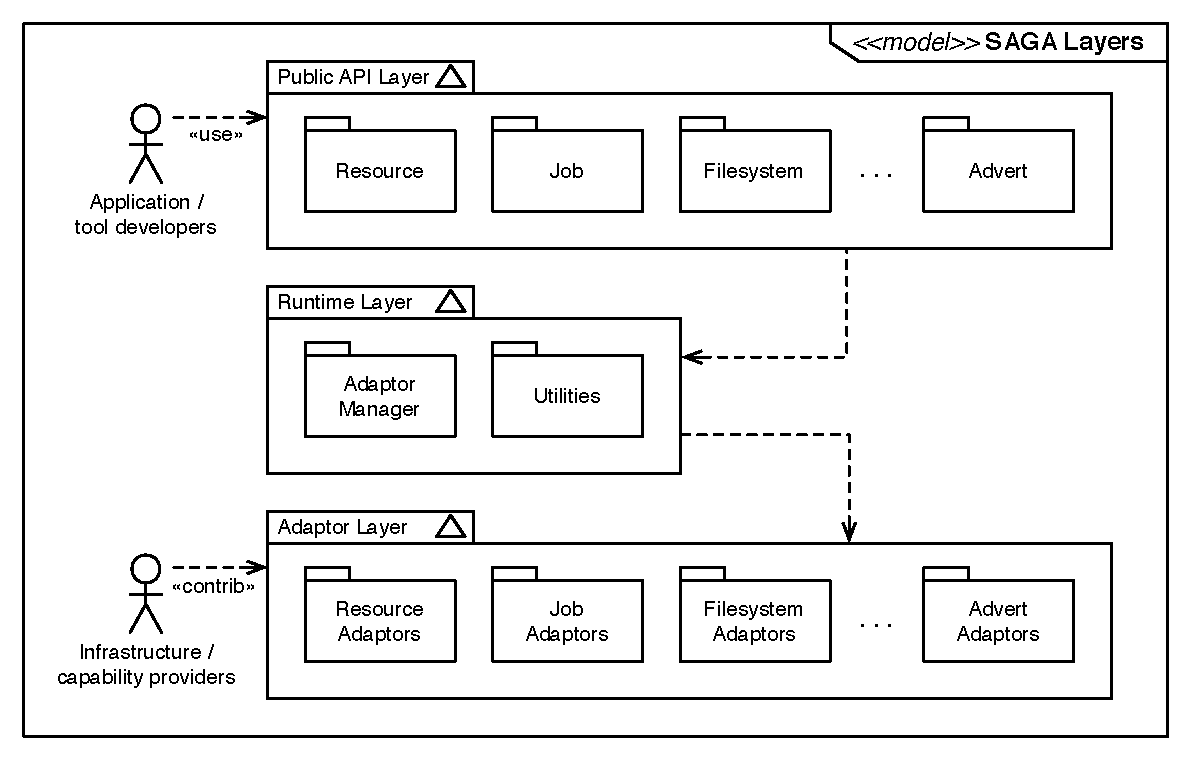
\includegraphics[width=0.9\textwidth]{figures/package_model.pdf} 
\caption{A package model for our SAGA implementation: a runtime layer provides the
coupling between the public API layer, which implements the SAGA interface, and
the adaptor layer, which implements the middleware bindings. The two actors represent 
the `user' of the interface layer, i.e., the application developer and the `user'
of the adaptor layer, i.e., infrastructure providers and service developers who
want to provide their community with a standardized interface.} 
\end{figure}


Having an architecture is only half the battle -- one also needs an
implementation of the architecture.


\subsection{Software Challenges}


\subsubsection{Language Challenges}

\subsubsection{External Dependencies}

\subsubsection{Packaging Challenges}

\subsubsection{Licensing}

\subsubsection{Performance}



\subsection{Testing, Deployment and Integration} 



\subsubsection{Integration with Middleware}
\subsubsection{Integration with Infrastructure}



%%%%%%%%%%%%%%%%%%%%%%%%%%%%%%%%%%%%%%%%%%%%%%%%%%%%%%%%%%%%%%%%%%%%%%
% 
\section{Applications and Frameworks}\todo{SJ}
\label{apps_and_frameworks}


Addressing this reiterates the importance of a well-defined general
purpose API that provides the basic distributed capabilities to serve
as building blocks for further applications and tools. The status of
the current workflow tools and enactment engines provides an
illustrative example~\cite{nsf-workflow,1196459}. Had SAGA or a
SAGA-like API been around, it is very likely that many distributed
workflow engines would have utilized SAGA (or parts thereof), instead
of proprietary solutions, to implement {\it common and basic}
distributed functionality, such as distributed job submission and
distributed file movement/management. SAGA's impact on the workflow
world can be seen through the consequences of its absence: in spite of
significant effort, workflow interoperability at multiple levels --
application, tools, enactment engines and components remains difficult
if not infeasible.  Significant effort has been invested towards
workflow interoperability at these different levels -- if nothing
else, providing post-facto justification of its importance.
Additionally, workflow capabilities and engines are typically tied to
specific tools and infrastructure (e.\,g.\ DAGMan-Condor) and require
the adaption of the application/usage modes to the workflow engine as
opposed to the other way around.



The situation now is potentially very different for emerging tools and
infrastructure such as Pilot-Jobs. A well defined API for distributed
applications in the form of Pilot-API now exists; a stable
implementation of it is on the horizon; the importance of
extensibility, interoperability and lessons from the workflow
experience have hopefully been learned and there is a willingness to
adopt and integrate...

%%%%%%%%%%%%%%%%%%%%%%%%%%%%%%%%%%%%%%%%%%%%%%%%%%%%%%%%%%%%%%%%%%%%%%
% 
\section{Discussion}\todo{All}

\subsection{Lessons Learned}

\subsubsection{Role of Standards?}

\paragraph{Importance of Standards for Interoperability and
    Integration}~

There are multiple routes to building system software for
infrastructure: for example, each project builds its own set of high
level abstractions for job and data management that are then targeted
at a variety of different backend systems such as PBS, Globus, Condor,
CREAM, etc. Similarly each middleware stack could develop specialized
code to integrate with each of many different other middleware stacks.

The first problem with this approach is that each project must build
and maintain what is essentially very similar software, resulting in
both a significant duplication of effort and the diversion of
intellectual resources that could better be used on the science
application into a fairly mundane programming task.  The second
problem is that software integration within an infrastructure is being
done ad-hoc and not designed to support integration across
infrastructure.

Using a standards-based approach mitigates these barriers to
interoperability and other problems in integrating components. When
developers use standard interfaces and implementations that mask the
diversity of back-end systems, they both free themselves from having
to implement the abstractions (including realizing the abstractions on
new backends as they become available), and give themselves the
freedom to easily switch from one implementation to another. Similarly
when a new resource implementation is added, middleware developers do
not need to modify their code with a whole new set of code paths to
deal with the new resource implementation.  SAGA is a prime example of
such a standards-based software that promotes both interoperability
within and across infrastructures.

A standards based approach is not by itself a guarantee of effective
system software/middleware integration or sustainable software --
there are many factors determining the outcome of such a complex
process. However, a standards based approach is an important
determinant and indicator of effectiveness and sustainability.  One
may argue that adherence to a standards-based software and development
is both an important funding mandate as well as technically expedient.  

Standards are, in our experience, relatively easy to introduce into
 existing development projects, and re thus likely to be enforceable
 on a timescale shorter than a complete radical overhaul of NSF’s
 ''software sustainability model''.

\subsection{Related Work}

\subsubsection{The Interface Standards Landscape}\label{interface_landscape}

\subsection{DCI and DA: The Road Ahead}

\subsubsection{Emergence of Clouds}

\subsubsection{Data as First-Class Entity}

\subsubsection{Application-Level Dynamism}

\subsubsection{Templatized MW-Stacks and Appliances}

\bibliographystyle{IEEEtran} 
\bibliography{saga_ogf,radical_rutgers}


\end{document}




